% System overview flowchart: DAW → PLL → Position/velocity mapping → Servo system
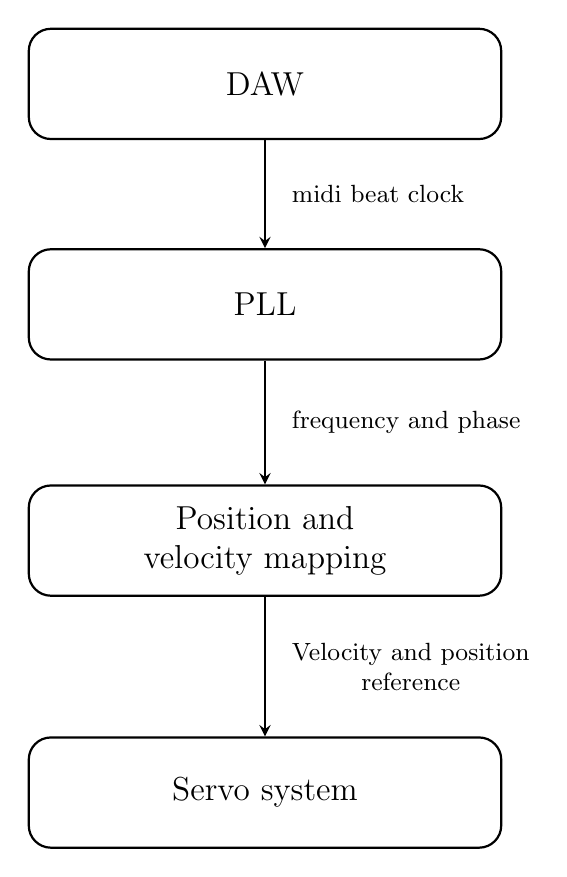
\begin{tikzpicture}[
	box/.style={
		draw, rounded corners=8pt, thick,
		minimum width=6cm, minimum height=1.4cm,
		align=center, font=\large
	},
	arr/.style={->, >=stealth, thick},
	lbl/.style={font=\small, align=center}
]

\node[box] (daw)     at (0,  0)   {DAW};
\node[box] (pll)     at (0, -2.8) {PLL};
\node[box] (mapping) at (0, -5.8) {Position and\\velocity mapping};
\node[box] (servo)   at (0, -9.0) {Servo system};

\draw[arr] (daw.south)     -- node[lbl, right=6pt] {midi beat clock}              (pll.north);
\draw[arr] (pll.south)     -- node[lbl, right=6pt] {frequency and phase}          (mapping.north);
\draw[arr] (mapping.south) -- node[lbl, right=6pt] {Velocity and position\\reference} (servo.north);

\end{tikzpicture}
